\section{Further Reference}
\label{reference_10}

\subsection{Abstract Machine}
\label{abstract_machine}

\subsection{Abstract Machine Notation}
\label{abstract_machine_notation}

\subsection{Arithmetic}
\label{arithmetic}

\subsection{Atelier B Provers}
\label{atelier_b_provers}

\subsection{Auto Prover}
\label{auto_prover}

The auto-prover can be configured by means of a preference page, which can be obtained as follows: press the "Window" button on the top tooolbar. On the coming menu, press the "Preferences" button. On the coming menu, press the "Event-B" menue, then the "Sequent Prover’, and finally the "Auto-Tactic" button. This yields the window in figure \ref{fig_ref_10_auto_prover_pref}.

\begin{figure}[!h]
\begin{center}
	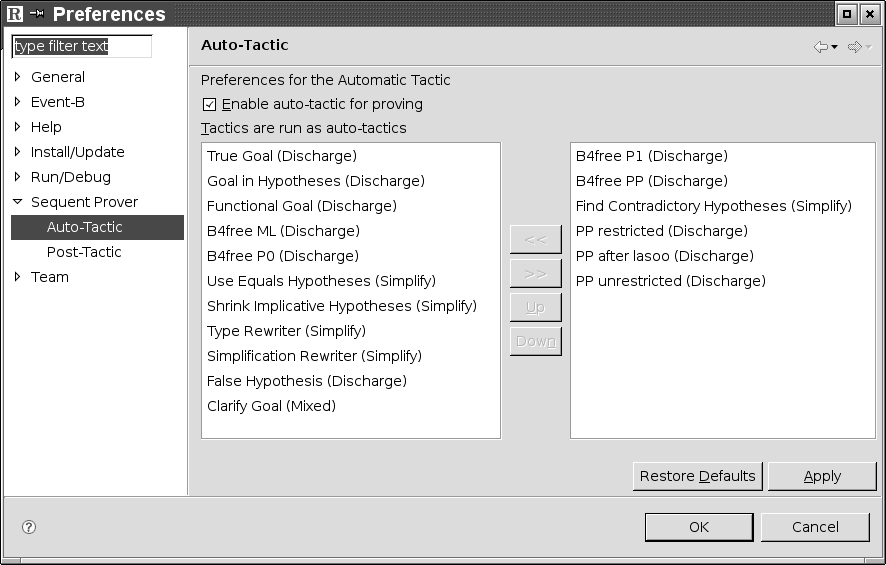
\includegraphics{img/reference/ref_10_auto_prover_pref.png}
	\caption{Auto Prover Preferences}
	\label{fig_ref_10_auto_prover_pref}
\end{center}
\end{figure}

On the left part you can see the ordered sequence of individual tactics composing the auto-prover, whereas the right part contains further tactics you can incorporate in the left part. By selecting a tactic you can move it from on part to the other or change the order in the left part. 

\subsection{Axiom}
\label{axiom}

\subsection{B}
\label{b}

A formal modeling notation.  Two dialects are classical B (\ref{classical_b}) and Event-B (\ref{event_b}).

\subsection{Camille}
\label{camille}

Camille is an alternative, text-based editor.  It can be installed through the Eclipse Install mechanism.  More information is available in the Rodin Wiki (\ref{rodin_wiki}).

\subsection{Classical B}
\label{classical_b}

\subsection{Constant}
\label{constant}

\subsection{Context}
\label{context}

\subsection{Customizing a perspective suitable for RODIN}
\label{customizing_a_perspective_suitable_for_rodin}

\marginpar{CONTENT MIGRATED FROM WIKI!}

So far, you needed two different perspectives to work with RODIN. But really, it is possible to work with only one perspective. In this section, we try to customize a perspective so that we do not need any other. If you have experience with customizing Eclipse perspectives, you may only want to read the next paragraph which contains a few thoughts about a good perspective for RODIN.


As a start, we should think about what we want the perspective to look like. The proving perspective already is pretty nice. We just could use little bit more editing space and the windows of the Event-B perspective. To create more space, we could move all windows that currently are on both sides of the editing area onto one side, as they never really need to be used simultaneously. For even a bit more space, we could dock all of these windows onto the so-called Fast View Bar, so that they disappear when they are not needed. Like that, there should be enough space to even work split-screen with different components, for example, we could have an abstract machine on one side of the editing surface, and the concrete machine on the other.


Most of the perspective editing is simply drag and drop. First of all, you need to find the Fast View Bar. Usually, it is at the bottom end of the Eclipse window. But it also can be on the side or hidden inside the Shortcut Bar. For our purposes, it probably is best to have it on the right side of the screen. Place it there by dragging it with the mouse. Now, add some items to it. To do that, press the New Fast View button on the bar. It might be useful to leave the Goal, the Problems and the Proof Control window at the bottom of the screen, as you may want them to stay open while editing. A good choice for the Fast view may be:

\begin{itemize}
	\item Project Explorer
	\item Obligation Explorer
	\item Search Hypothesis
	\item Cache Hypothesis
	\item Proof Tree
	\item Proof Information
	\item Progress Window
\end{itemize}

All of the windows that you cannot create directly when clicking on the New Fast View Bar can be found in Others/General. Once you are done, the window should look like in Figure \ref{fig_ref_10_customizing}. Click on “Save Perspective As…” in the Window menu to save the perspective.

\begin{figure}[!h]
\begin{center}
	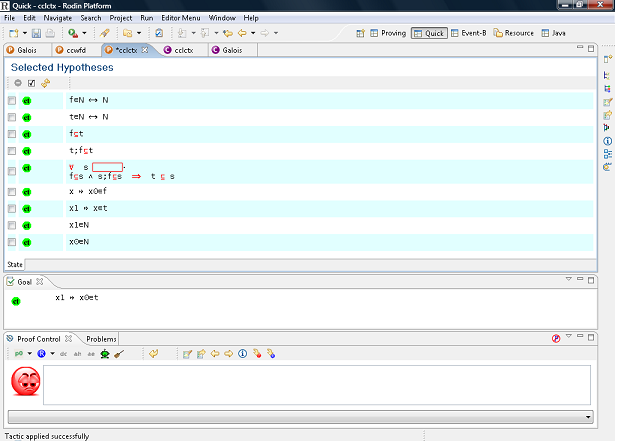
\includegraphics{img/reference/ref_10_customizing.png}
	\caption{Our self-made Quick perspective}
	\label{fig_ref_10_customizing}
\end{center}
\end{figure}

\subsection{Data Refinement}
\label{data_refinement}

\subsection{Datatypes}
\label{datatypes}

List of Event-B datatypes

\subsection{Deadlock}
\label{deadlock}

\subsection{Deploy}
\label{deploy}

The Deploy Project funded the Rodin project in part.  More information at \url{http://www.deploy-project.eu/}.

\subsection{Eclipse}
\label{eclipse}

- Eclipse Definition

- Pointers to Web Tutorials, etc.

\subsection{Editor View}
\label{editor_view}


\subsection{Event}
\label{event}

Definition event

\subsection{Event-B}
\label{eventb}

Event-B is a formal method (\ref{formal_method}) for system-level modelling and analysis. Key features of Event-B are the use of set theory (\ref{set_theory}) as a modelling notation, the use of refinement (\ref{refinement}) to represent systems at different abstraction levels and the use of mathematical proof to verify consistency between refinement levels.

\paragraph{See Also:}
\begin{itemize}
\item \url{http://www.event-b.org}
\end{itemize}

\subsection{Event-B Component}
\label{eventb_component}

Machines (\ref{machine}) and Contexts (\ref{context}) are components.

\subsection{Event-B Explorer}
\label{eventb_explorer}

The View showing the Event-B projects and their content.  In the default Event-B perspective, it is the slim browser on the left edge of the Workspace.  If it is missing, make sure that you use the correct perspective.  You can explicitly enable it with \textsf{Windows $\rangle$ Show View... $\rangle$ Event-B Explorer}.

\subsection{First Order Predicate Calculus}
\label{first_order_predicate_calculus}


\subsection{Formal Method}
\label{formal_method}

\subsection{Gluing Invariant}
\label{gluing_invariant}

\subsection{Goal View}
\label{goal_view}

\subsection{Guard}
\label{guard}

\subsection{IDE}
\label{ide}

Integrated Development Environment

\subsection{Initialization}
\label{initialization}

Every machine has a special event \texttt{INITIALIZATION} that will be used to initialize the machine's state.

TODO: Determinism, refinement.

\subsection{Label}
\label{label}

\subsection{Machine}
\label{machine}

\subsection{Mathematical Notation}
\label{mathematical_notation}

\subsection{Menu Bar}
\label{menu_bar}

\subsection{Model Checker}
\label{model_checker}

\subsection{Naming Convention}
\label{naming_convention}

In this subsection we describe a recommended naming convention.  Good naming conventions save time -- and nerves.

\subsection{Non-Deterministic}
\label{non_deterministic}

\subsection{Outline View}
\label{outline_view}

\subsection{P0 Prover}
\label{p0_prover}

\subsection{Partition}
\label{partition}

\subsection{Proof Control View}
\label{proof_control_view}

\subsection{Proof Obligation}
\label{proof_obligation}

\subsection{Proof Tree View}
\label{proof_tree_view}

\subsection{Plugin}
\label{plugin}

\subsection{Refinement}
\label{refinement}

\begin{description}
	\item[Horizontal Refinement]
	\item[Vertical Refinement]
	\item[Data Refinement]
\end{description}

\paragraph*{See also:}
\begin{itemize}
\item Data refinement in the trafficlight tutorial (\ref{tutorial:data_refinement})
\end{itemize}

\subsection{Rodin Wiki}
\label{rodin_wiki}

\url{http://wiki.event-b.org/}

\subsection{Structural Editor}
\label{structural_editor}

\subsection{Symbols View}
\label{symbols_view}

\subsection{Predicate Logic}
\label{predicate_logic}

\subsection{ProB}
\label{prob}

ProB is an animator and model checker for the B-Method. It allows fully automatic animation of many B specifications, and can be used to systematically check a specification for errors. 

ProB is available as a Rodin Plugin.

\paragraph*{See also:}
\begin{itemize}
\item ProB Website: \url{http://www.stups.uni-duesseldorf.de/ProB}
\item In the tutorial: Section~\ref{tut:prob}
\end{itemize}


\subsection{Project}
\label{project}

\marginpar{CONTENT MIGRATED FROM WIKI!}

\subsubsection{Project Constituents and Relationships}

The primary concept in doing formal developments with the Rodin Platform is that of a project. A project contains the complete mathematical development of a Discrete Transition System. It is made of several components of two kinds: machines and contexts. Machines contain the variables, invariants, theorems, and events of a project, whereas contexts contain the carrier sets, constants, axioms, and theorems of a project. Figure \ref{fig_ref_10_project1} shows an overview.

\begin{figure}[!h]
\begin{center}
	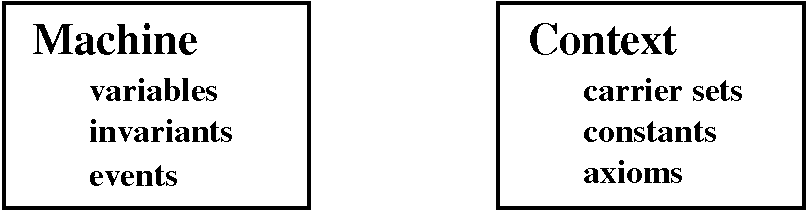
\includegraphics{img/reference/ref_10_project1.png}
	\caption{Overview Machine and Context}
	\label{fig_ref_10_project1}
\end{center}
\end{figure}

We remind the reader of the various relationships existing between machines and contexts. This is illustrated in the following figure. A machine can be "refined" by another one, and a context can be "extended" by another one (no cycles are allowed in both these relationships). Moreover, a machine can "see" one or several contexts. A typical example of machine and context relationship is shown in figure \ref{fig_ref_10_project2}. 

\begin{figure}[!h]
\begin{center}
	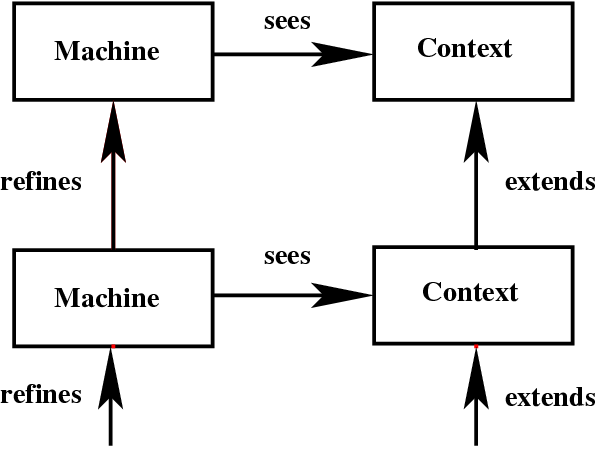
\includegraphics{img/reference/ref_10_project2.png}
	\caption{A typical example of machine and context relationship}
	\label{fig_ref_10_project2}
\end{center}
\end{figure}

\subsection{Proof Obligation Labels}
\label{po_labels}

\subsection{Propositional Calculus}
\label{propositional_calculus}

\subsection{Proof Purger Interface}
\label{proof_purger_interface}

\marginpar{CONTENT MIGRATED FROM WIKI!}

\subsubsection{Purpose}

Proofs are stored in proof files. Each time a new proof obligation is generated by the tool, a corresponding (initially empty) proof is created. However, proofs are never removed automatically by the Rodin platform. As time passes and a model is worked out, obsolete proofs (e.g., proofs that do not have a corresponding proof obligation anymore) accumulate and clutter proof files.

The purpose of the proof purger is to allow the user to delete obsolete proofs. 

\subsubsection{Why proofs become obsolete}

Proof obligations are named after the main elements related to it, such as events and invariants. Therefore, each time such an element is renamed manually, the corresponding proof obligations get a new name. However, the existing proof is not renamed, and a new proof gets created with the new name.

Therefore, after a lot of model editing, there are more and more obsolete proofs stored in proof files.

\subsubsection{Selecting purge input}

In any view, right-clicking an Event-B project or file will display a popup menu, containing a Purge Proofs... entry. If several files or projects (or both) are selected, purging will apply to all of them.

Firstly, the proof purger tries to find obsolete proofs in the selection. If no obsolete proof is found, a message will pop up telling that no proof needs to be purged. Otherwise, a new window will pop up displaying a list of all POs that are considered obsolete, that is all proofs that exist in some proof file and that do not have any corresponding proof obligation. 

\subsubsection{Choosing proofs to delete}

\begin{figure}[!h]
\begin{center}
	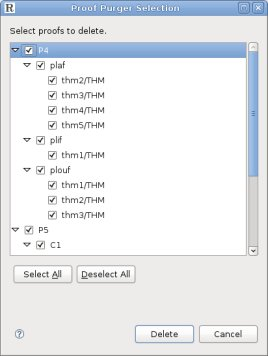
\includegraphics{img/reference/ref_10_proof_purger.png}
	\caption{Proof Purger Selection Window}
	\label{fig_ref_10_proof_purger}
\end{center}
\end{figure}

For the moment, nothing has been erased. The new window (see figure \ref{fig_ref_10_proof_purger}) shows obsolete proofs and offers to choose among them which ones should be deleted. One may wish to keep some of them, knowing they might be useful in the future.

Once the selection has been decided, clicking the Delete button will actually delete selected proofs from proof files. Files becoming empty will be deleted as well.

\subsubsection{Caution}

Proof purging shall not be performed on models that are not in a stable state. For instance, it should not be applied to a model that bears some errors or warnings issued by the type checker. This is because, in case of errors and warnings, it can happen that not all proof obligations are generated. Therefore, some proofs could be considered wrongly as obsolete.

\subsection{Relation}
\label{relation}

\subsection{Rodin}
\label{rodin}

\marginpar{CONTENT MIGRATED FROM WIKI!}

The Rodin Platform is an Eclipse-based IDE for Event-B that provides effective support for refinement and mathematical proof. The platform is open source, contributes to the Eclipse framework and is further extendable with plugins. 

\subsection{Rodin Download}
\label{rodin_download}

Download Page: http://sourceforge.net/projects/rodin-b-sharp/files/Core\_Rodin\_Platform/


\subsection{Rodin Platform}
\label{rodin_platform}



\subsection{Rodin Problems View}
\label{rodin_problems_view}


\subsection{Rodin Nature}
\label{rodin_nature}

Eclipse Projects can have one or more natures to describe their purpose.  The GUI can then adapt to their nature.  Rodin Projects must have the Rodin-Nature.  If you create an Event-B project, it automatically has the right nature.  If you want to modify an existing project, you can edit the \texttt{.project} file and add the following XML in the \texttt{<natures>} section:

\pencil{
\texttt{<nature>org.rodinp.core.rodinnature</nature>}
}

\subsection{Sequents}
\label{sequents}

A sequent stands for something we want to prove.

Sequents are of the following form

$H \vdash G$

where H is the set of hypotheses (predicates) and G is the goal (a predicate in the mathematical language).

The meaning of the above sequent is that: Under the hypotheses H, prove the goal G. 

\subsection{Sees}
\label{sees}

\subsection{Set}
\label{set}

\subsection{Set Theory}
\label{set_theory}

... Set Theory Definition ...

\subsection{Temporal Logic}
\label{temporal_logic}

\subsection{Theorem}
\label{theorem}

\subsection{Tool Bar}
\label{tool_bar}

\subsection{Undischarged Proof Obligations}
\label{undischarged_proof_obligations}

\subsection{Upgrade}
\label{Upgrade}

\subsection{Variant}
\label{variant}

\marginpar{CONTENT MIGRATED FROM WIKI!}

The variant section appears in a refined machine (section 1) containing some convergent or anticipated events (section 2). This machine section contains either a natural number expression which must be decreased by each convergent event and not be increased by each anticipated event, or a finite set expression which must be made strictly smaller by each convergent event or not made greater by each anticipated events. 

\subsection{Well-definedness in Event-B}
\label{well_definedness_in_event_b}

\marginpar{CONTENT MIGRATED FROM WIKI! (http://wiki.event-b.org/index.php/Well-definedness\_in\_Event-B)}

In classical set theory (see, e.g., H. B. Enderton, Elements of Set Theory, Academic Press, 1977), the formula $1\div 0 = 1\div 0$ is true, because $1\div 0$ denotes some set or number; we just do not know which one. In Event-B however, $1\div 0$ does not denote a particular set or number and therefore receives a specialized treatment. The formula $1\div 0 = 1\div 0$ is then neither true nor false; it is ill-defined.

Formally, there is a syntactic transformation $\mathcal{D}$ mapping terms and formulae to a well-definedness condition, which itself is a formula. The term or formula E is well-defined iff $\mathcal{D}(E)$ can be proved and otherwise ill-defined. For example:

    $\mathcal{D}(x\div y) \defi y \neq 0.$
    $\mathcal{D}(\phi\lor\psi)\defi(\mathcal{D}(\phi)\land\mathcal{D}(\psi))\lor(\mathcal{D}(\phi)\land\phi)\lor(\mathcal{D}(\psi)\land\psi).$
    $\mathcal{D}(y=0 \lor (x\div y) * y = x)$ is equivalent to $y\neq0 \lor y = 0, whence y\neq0\limp(x\div y)*y=x$ is well-defined.
    Because $\mathcal{D}$ preserves the symmetry of disjunction, $(x\div y)*y=x \lor y = 0$ is also well-defined. 

Well-definedness is similar to well-typedness, just that checking well-definedness is undecidable, because it involves finding a proof.

As $\mathcal{D}(E)$ in the worst case grows exponentially in the size of E, it is not computed directly in the Rodin platform. Instead another syntactic transformation $\mathcal{L}$ is defined, and $\mathcal{D}(E)$ is approximated by $\mathcal{L}(E)$. In the case of disjunction, $\mathcal{L}(\phi\lor\psi)\defi\mathcal{L}(\phi)\land(\lnot\phi\limp\mathcal{L}(\psi))$, which is equivalent to the first two disjuncts of $\mathcal{D}(\phi\lor\psi)$. One may therefore view $\mathcal{L}(E)$ as an incomplete strategy for proving $\mathcal{D}(E)$. Approximating $\mathcal{D}$ by $\mathcal{L}$ is sound, because $\mathcal{L}(E)\limp\mathcal{D}(E)$ is always provable. 

Nomenclature

In this article the following nomenclature is used:

    1 + 1 = 2 is a formula.
    1 + 1 is a term.
    + is an operator.
    = is a predicate. 

In other places (but not in this wiki-page), 1 + 1 = 2 is called predicate and 1 + 1 expression.
[edit] D-Well-Definedness
[edit] Definition

We associate with each operator f a domain condition $\mathcal{DOM}(f)$. Informally, the domain condition of an operator determines which terms the operator may be applied to. Formally, if $f(\mathbf{t})$ is a term, then $\mathcal{DOM}(f)(\mathbf{t})$ is a formula. Intuitively, if $f(\mathbf{t})$ is a (well-typed) term, $\mathcal{DOM}(f)(\mathbf{t})$ is true if and only if $\mathbf{t}$ belongs to the "intended domain" of f.

For example,

    $\mathcal{DOM}(\div)(t, u) \defi u \neq 0$,
    $\mathcal{DOM}(\mathrm{app})(r,x)) \defi x \in \dom(r) \land r \in A \pfun B$, assuming that r is of type $\pow(A \times B)$. 

Here the operator app takes a function r and a value x and returns the result of applying r to x.

The various domain conditions can be found in the Event-B mathematical language description.

Based on the domain conditions, we associate with each term or formula E a well-definedness condition $\mathcal{D}(E)$, respectively. Well-definedness conditions are formulae as follows:
(x ranges over variables, f over operators, p over predicates, $\mathbf{t}$ over sequences of terms of length $|\mathbf{t}|$, and $φ$, $ψ$ over formulae. All terms and formulae are well-formed and well-typed.)

    $\mathcal{D}(x)\defi \btrue$,
    $\mathcal{D}(f(\mathbf{t}))\defi \mathcal{DOM}(f)(\mathbf{t}) \land \bigwedge_{i=1}^{|\mathbf{t}|} \mathcal{D}(t_i)$,
    $\mathcal{D}(\{x\mid \phi\})\defi \forall x\qdot \mathcal{D}(\phi)$,
    $\mathcal{D}(p(\mathbf{t}))\defi \bigwedge_{i=1}^{|\mathbf{t}|} \mathcal{D}(t_i)$,
    $\mathcal{D}(\btrue) \defi \mathcal{D}(\bfalse) \defi \btrue$,
    $\mathcal{D}(\lnot\phi) \defi \mathcal{D}(\phi)$,
    $\mathcal{D}(\phi\land\psi)\defi (\mathcal{D}(\phi) \land \mathcal{D}(\psi)) \lor (\mathcal{D}(\phi) \land \lnot\phi) \lor (\mathcal{D}(\psi) \land \lnot\psi)$,
    $\mathcal{D}(\phi\lor\psi)\defi (\mathcal{D}(\phi) \land \mathcal{D}(\psi)) \lor (\mathcal{D}(\phi) \land \phi) \lor (\mathcal{D}(\psi) \land \psi)$,
    $\mathcal{D}(\phi\limp\psi)\defi (\mathcal{D}(\phi) \land \mathcal{D}(\psi)) \lor (\mathcal{D}(\phi) \land \lnot\phi) \lor (\mathcal{D}(\psi) \land \psi)$,
    $\mathcal{D}(\phi\leqv\psi)\defi \mathcal{D}(\phi) \land \mathcal{D}(\psi)$,
    $\mathcal{D}(\forall x\qdot \phi)\defi (\forall x \qdot \mathcal{D}(\phi)) \lor (\exists x \qdot \mathcal{D}(\phi) \land \lnot \phi)$,
    $\mathcal{D}(\exists x\qdot \phi)\defi (\forall x \qdot \mathcal{D}(\phi)) \lor (\exists x \qdot \mathcal{D}(\phi) \land \phi)$. 

A constant c is an operator of arity zero and therefore has the well-definedness condition $\mathcal{DOM}(c)()$, which equals $\btrue$ for all currently supported constants.

Intuitively, the well-definedness condition of a term or formula is true if and only if the term or formula can be evaluated without applying an operator to an argument outside of its domain.

Well-Definedness and Provability

Recall that the set of provable sequents is the smallest set of sequents such that if all antecedents of some inference rule are provable then so is the consequent. See Inference Rules and All Rewrite Rules for an incomplete list of rules that may be used to prove a sequent. (Here we view rewrite rules also as inference rules.) In the future, more rules will be added to this list so that more sequents will be provable. In particular, the following rules may also be used to prove a sequent:

TODO FORMULA!

A formula $φ$ is provable if and only if the sequents $\vdash\phi and \vdash\mathcal{D}(\phi)$ are provable.

It can be checked (see F. D. Mehta, Proofs for the working engineer, Diss. ETH Zurich, 2008) that for each term or formulae E the formula $\mathcal{D}(E)$ is provable iff $\vdash\mathcal{D}(E)$ is provable. We therefore say that a term or formula is well-defined iff its well-definedness condition is provable. A term or formula is ill-defined iff it is not well-defined.

Informally, well-definedness conditions appear in two ways during proofs:

    When proving a formula, we also have to prove its well-definedness.
    When proving a sequent, we may always assume that the hypotheses and the goal of the sequent are well-defined. 

L-Well-Definedness

As $\mathcal{D}(E)$ in the worst case grows exponentially in the size of E, $\mathcal{D}$ is never evaluated explicitely in the Rodin platform. To avoid evaluating $\mathcal{D}$, we define the syntactic transformation $\mathcal{L}$ as follows:
(Again, x ranges over variables, f over operators, p over predicates, $\mathbf{t}$ over sequences of terms of length $|\mathbf{t}|$, and $φ$, $ψ$ over formulae. All terms and formulae are well-formed and well-typed.)

    $\mathcal{L}(x)\defi \btrue$,
    $\mathcal{L}(f(\mathbf{t}))\defi \mathcal{DOM}(f)(\mathbf{t}) \land \bigwedge_{i=1}^{|\mathbf{t}|} \mathcal{L}(t_i)$,
    $\mathcal{L}(\{x\mid \phi\})\defi \forall x\qdot \mathcal{L}(\phi)$,
    $\mathcal{L}(p(\mathbf{t}))\defi \bigwedge_{i=1}^{|\mathbf{t}|} \mathcal{L}(t_i)$,
    $\mathcal{L}(\btrue) \defi \mathcal{L}(\bfalse) \defi \btrue$,
    $\mathcal{L}(\lnot\phi) \defi \mathcal{L}(\phi)$,
    $\mathcal{L}(\phi\land\psi)\defi \mathcal{L}(\phi) \land (\phi \limp \mathcal{L}(\psi))$,
    $\mathcal{L}(\phi\lor\psi)\defi \mathcal{L}(\phi) \land (\lnot\phi \limp \mathcal{L}(\psi))$,
    $\mathcal{L}(\phi\limp\psi)\defi \mathcal{L}(\phi) \land (\phi \limp \mathcal{L}(\psi))$,
    $\mathcal{L}(\phi\leqv\psi)\defi \mathcal{L}(\phi) \land \mathcal{L}(\psi)$,
    $\mathcal{L}(\forall x\qdot \phi)\defi \forall x\qdot \mathcal{L}(\phi)$,
    $\mathcal{L}(\exists x\qdot \phi)\defi \forall x\qdot \mathcal{L}(\phi)$. 

Only Conditions 7, 8, 9, 11, 12 differ from the corresponding conditions in the definition of $\mathcal{D}$.

The two syntactic transformations $\mathcal{D}$ and $\mathcal{L}$ are related as follows:

    $\mathcal{L}(E) \limp \mathcal{D}(E)$ is provable for every term or formula E.

Based on this observation, the transformation $\mathcal{D}$ is avoided in Rodin's proof calculus as follows:

    To prove φ, the user has to prove $\vdash\phi$ and $\vdash\mathcal{L}(\phi)$.
    If an inference rule contains well-definedness conditions $\mathcal{D}(E)$, the rule may not be added to the list of rules available in Rodin.
        If the well-definedness conditions $\mathcal{D}(E)$ only appear as goals of antecedents and hypotheses of the consequent, the rule obtained by replacing $\mathcal{D}(E)$ by $\mathcal{L}(E)$ is made available in Rodin. For example, instead of adding the rule

        TODO FORMULA!
        the rule 
        TODO FORMULA!
        is added to the list of inference rules. 

        If a well-definedness condition $\mathcal{D}(E)$ appears as a hypothesis of an antecedent or as the goal of the consequent, the rule may not be added to the list of rules available in Rodin. Therefore the above rules (*) are unavailable in Rodin. 

Note that avoiding $\mathcal{D}$ in Rodin's proof calculus is not necessary for soundness; it is just a way of making sequents arising in proofs smaller. The price of avoiding $\mathcal{D}$ in Rodin's proofs is that some formulae and sequents become unprovable.
[edit] Distinction between D and L

As $\mathcal{L}(E)$ is stronger than $\mathcal{D}(E)$, mixing them up easily leads to inconsistency in Rodin's proof calculus. To help the reader differentiate between the two syntactic transformations $\mathcal{D}$ and $\mathcal{L}$, we provide a summary of what is used where:

    In the documentation of Inference rules (Inference Rules and All Rewrite Rules), "WD" refers to $\mathcal{L}$.
    In the Rodin source code, the term "well-definedness predicate" refers to $\mathcal{L}(E)$, and (at the time of writing) the API of org.eventb.core.ast provides no method for computing $\mathcal{D}$.
    In Rodin, the goal of a well-definedness proof obligation is created by $\mathcal{L}$.
    The above rules (*) are sound, but the analog rules with $\mathcal{D}$ replaced by $\mathcal{L}$ are not, and they may therefore neither be added to the proof calculus nor be used to justify new inference rules. 

[edit] Design Decisions Revisited

In the following, we review some properties of the syntactic transformation $\mathcal{DOM}$, which should be preserved when introducing new operators and predicates in Event-B. We also list some properties of $\mathcal{D}$ and $\mathcal{L}$ to illustrate some design decisions underlying their definitions.
[edit] Important Properties of DOM

Technically, domain conditions map sequences of terms to formulae. But not every such mapping may be used as a domain condition.

    Only variables appearing in the sequence $\mathbf{x}$ of variables appear free in $\mathcal{DOM}(f)(\mathbf{x})$.
    $\mathcal{DOM}(f)(\mathbf{t}) \defi \mathcal{DOM}(f)(\mathbf{x})[\mathbf{x}\bcmeq\mathbf{t}]$.
    $\mathcal{DOM}(f)(\mathbf{x})$ syntactically only contains definite operators. An operator f is definite iff $\mathcal{DOM}(f)(\mathbf{x})\defi\btrue$ for every sequence $\mathbf{x}$ of variables of appropriate length and type. 

Property 3 ensures that $\mathcal{D}(E)$ is provable if and only if $\vdash\mathcal{D}(E)$ is provable. In the future, Property 3 may be replaced by a weaker version.
[edit] Important Properties of D and L
[edit] L is stronger than D

$\mathcal{L}(E) \limp \mathcal{D}(E)$ is provable for each term or formula E.
[edit] Monotonicity

We define the order $\sqsubseteq$ on terms and formulae by

    $t \sqsubseteq u iff \mathcal{D}(t)\limp t=u$ is provable, and
   $ \phi\sqsubseteq\psi iff \mathcal{D}(\phi)\limp (\phi\leqv\psi) is provable$. 

Then, $\mathcal{D}$ has the following monotonicity properties (TODO: add citation):
(u, v are terms, x is a variable, ψ, χ are formulae, E is a term or a formula, and p is a position in E.)

    If $u \sqsubseteq v, then E[x\bcmeq u] \sqsubseteq E[x\bcmeq v]$.
    If $\psi \sqsubseteq \chi, then E_p[\psi] \sqsubseteq E_p[\chi]$.

Here, Ep[ψ] denotes the term or formula obtained by replacing the subformula at position p in E by ψ. We assume that bound variables of E do not appear free in ψ or χ, which can be achieved by consistent renaming of variables.

The above monotonicity properties are crucial for the soundness of several rewrite rules, such as t * 0 $\defi 0$.

It is possible to prove similar monotonicity properties for $\mathcal{L}$ but monotonicity of $\mathcal{L}$ is not necessary for soundness of any inference rule.
[edit] Strictness

We have decided to make operators strict, i.e., if some element in the list of terms $\mathbf{t}$ is ill-defined, then so is $f(\mathbf{t})$, where f is an operator. Predicates are also strict.

The strictness property can be dropped without making any inference rule unsound, as long as the monotonicity properties of the previous section are preserved. An example for a non-strict operator retaining the monotonicity property is lazy multiplication mult: the term mult(t,u) denotes the same value as t * u if both t and u are well-defined, it denotes 0 if either t or u denotes 0, and it is ill-defined otherwise.
[edit] Predicates and Sets are Definite

We have decided to make predicates definite, i.e., a formula $p(t)$ is well-defined provided each element of $t$ is. Therefore, sets are also definite, i.e., $t \in A$ is well-defined provided t and A are.

It may be possible to allow for indefinite predicates and sets without compromising soundness of the proof calculus. In that case, it may be desirable to retain soundness of the following rewrite rules:
$p(t) \defi t \in \{x\mid p(x)\}$
$t\in\{x\mid p(x)\} \defi p(t)$
(t is a term, p a predicate, and x a variable.) 

\subsection{Witness}
\label{witness}

When a concrete event refines an abstract one which is parameterized, then all abstract parameters must receive a value in the concrete event. Such values are called the witnesses. Each witness is labelled with the concerned abstract parameter. The witness is defined by a predicate involving the abstract parameter. Most of the time, this predicate is a simple equality. Next is an example showing two witnesses. On the left hand side we have an abstract event named pass with two parameters. On the right hand side we have a concrete event named new\_pass refining pass 

$\begin{array}{l} \texttt{pass} \ \ \defi \\ \quad \textbf{any} \\ \quad \quad p \\ \quad \quad l \\ \quad \textbf{where}\\ \quad \quad grd1: \ \ {p \mapsto l \,\in\, aut}\\ \quad \quad grd2: \ \ sit(p)\mapsto l \,\in\, com \\ \quad \textbf{then} \\ \quad \quad act1: \ \ sit(p) \,:=\, l \\ \quad \textbf{end} \end{array}
\begin{array}{l} \texttt{new\_pass} \ \ \defi \\ \quad \textbf{refines} \\ \quad \quad \texttt{pass} \\ \quad \textbf{any} \\ \quad \quad d \\ \quad \textbf{where}\\ \quad \quad grd1: \ \ \ d \,\in\, ran(dap) \\ \quad \textbf{with} \\ \quad \quad p: \ \ \ p=dap^{-1}(d) \\ \quad \quad l: \ \ \ l=dst(d) \\ \quad \textbf{then} \\ \quad \quad act1: \ \ sit(dap^{-1}(d)) \,:=\, dst(d) \ \\ \quad \quad act2: \ \ dap \,:=\, dap \ransub \{d\} \\ \quad \textbf{end} \end{array} $

When the concrete event is also parameterized then an abstract parameter which is the same as a concrete need not be given an explicit witness: it is always the corresponding concrete parameter.

The initialisation event sometimes needs witnesses, in this case do not forget to use the after value of variable (x'). 

\subsection{Wizard}
\label{wizard}

\subsection{Zip File}
\label{zip_file}


